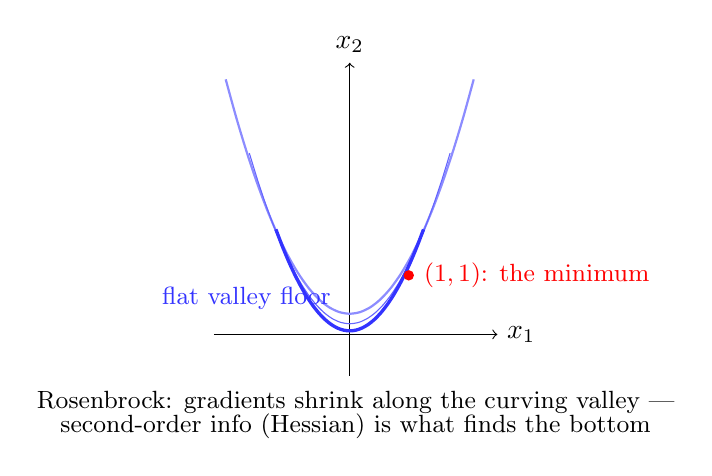
\begin{tikzpicture}[scale=0.75]
% banana valley: x2 = x1^2 curve; contours nested parabola-ish
\draw[->] (-2.3,0)--(2.5,0) node[right]{$x_1$};
\draw[->] (0,-0.7)--(0,4.6) node[above]{$x_2$};
\draw[domain=-2.1:2.1,smooth,variable=\x,blue!45,thick] plot (\x,{0.9*\x*\x+0.35});
\draw[domain=-1.7:1.7,smooth,variable=\x,blue!60] plot (\x,{\x*\x+0.18});
\draw[domain=-1.25:1.25,smooth,variable=\x,blue!80,very thick] plot (\x,{1.1*\x*\x+0.06});
\fill[red] (1,1) circle (2.5pt) node[right=2pt]{\small $(1,1)$: the minimum};
\node[blue!80] at (-1.75,0.62) {\small flat valley floor};
\node at (0.1,-1.15) {\small Rosenbrock: gradients shrink along the curving valley ---};
\node at (0.1,-1.55) {\small second-order info (Hessian) is what finds the bottom};
\end{tikzpicture}
